%! Author = chrystal
%! Date = 03.12.19

% Preamble
\documentclass[11pt]{article}

% Packages
\usepackage{amsmath}

\chapter{Standardizing Data}

\begin{section}{Normal distribution}

    \paragraph{A normal distribution follows certain distribution rules}

    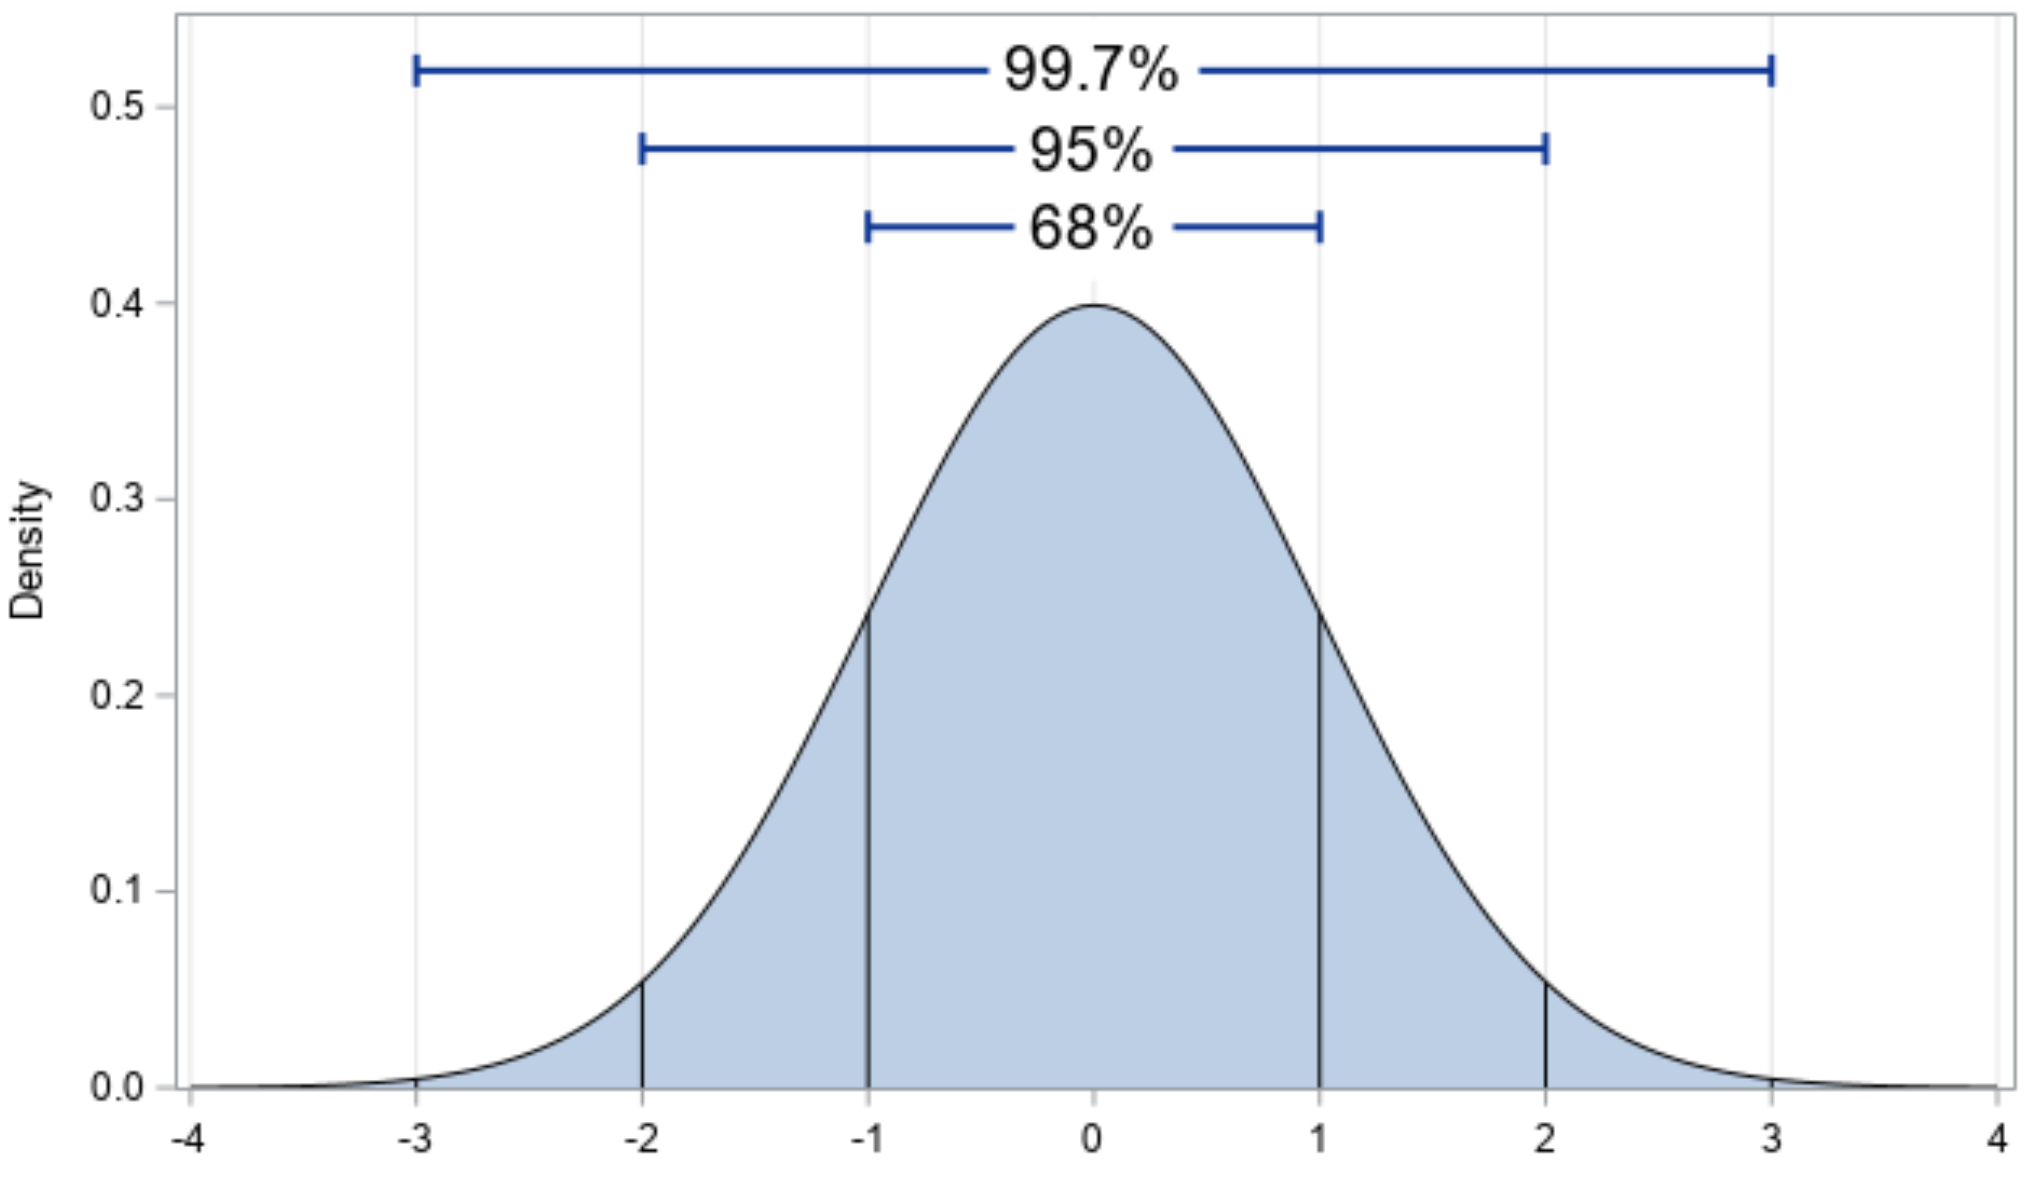
\includegraphics{../assets/normal-distribution.png}

    \paragraph{Z-scores} Subtract a given value from its population mean and divide by the standard deviation.
    The z-mean of the z-distribution is 0, and the z-standard deviation is 0.
    If you have standardized the data, it is easy to determine the
    probabilities of observing this such a value or a smaller/greater one using a standard normal distribution table

    $$z = (X - \mu ) \sigma $$

    \subsection{Hypothesis Testing}

    \paragraph{1. Define two states of the world} \textbf{H_0} is the state of the world where nothing significant is happening and everything is distributed normally
    - if something interesting is happening, it is due to random variation.
    \textbf{H_1} is the state of the world where something significant is happening

    \paragraph{\textit{Example}} \textit{
    Do men prefer cats over dogs if from a random sample of 100 men, 60 have cats?
    \textbf{H_0: } Man have as many dogs as cats $\rightarrow \frac{man_cat}{men_pet} = \frac{man_{dog}}{men_pet} \rightarrow catsPercentage = 50\%$
    \textbf{H_1: } Man have as not as many dogs as cats $\rightarrow \frac{man_cat}{men_pet} \neq \frac{man_{dog}}{men_pet} \rightarrow catsPercentage \neq 50\%$

    Imagine out of 100.000 men, 100 samples with each 100 men get drawn by random. The range of these samples may vary to a point to find 100 cat owners.
    The Hypothese test will tetermine how likely the given sample is compared to a normal distribution.
    }

    \paragraph{2. Calculate z value for H_0} $p$ = size of the sample population, \pi = test value, $n=$ sample size
    $$
    z=\frac{p-\pi}{\sigma_p} \sigma_p = \sqrt{\frac{\pi \time (1-\pi)}{n}}
    $$

    \paragraph{Example (continued)} $\sigma_p = \sqrt{\frac{0.5 \time (1-0.5)}{100}} z=\frac{p-0.5}{0.05} = 2.0$

    \paragraph{3. Calculating the p-value (significance level)} Calculate the right and left extreme value to determine the probability of a value more extreme than in H_0.
    The smaller the p value, the less likely we make a Type I error
    $$ P(z \leq z_{H0} | H_o true) = p-value $$

    \paragraph{Example (continued)} $p(z \leq 2) + p(z < 2) = 0.0455 \rightarrow p(z \leq 2 | H_0 true) = 0.0455$

    \paragraph{4. Checking Significance}
    If $p \leq 0.05$, H0 is rejected $\rightarrow$ the parameter is significantly different from a specific value (one sample) or across groups (two or more samples).
    If $0.5 \leq p \leq 0.1$ H0 is rejected but marginally $\rightarrow$ the parameter is marginally significantly different from a specific value or across groups.
    If $p > 0.1$, H0 is not rejected $\rightarrow$ the parameter is not statistically different from a specific value or across groups.

    If H_0 is rejected, bu H_0 is true $\rightarrow$ Type 1 Error (False positive)
    If H_0 is accepted, bu H_0 is false $\rightarrow$ Type 2 Error (False negative)

    \paragraph{Example (continued)} Reject H_0, accept H_1

    \subsection{Two sided and one sided Hypothesis testing}

    \paragraph{Two-sided tests}
    \textbf{H_0} the parameter (e.g., mean, proportion) of the variable is equal to a specific value(s) (one sample) or Across different groups (two or more samples).
    \textit{X and Y are equally liked; the average is equal to 40 0...}
    \textbf{H_1} the parameter of the variable is different to the specific value(s) or Across different groups.
    \textit{X and Y are not equally liked; the average is not 40 ...}

    \paragraph{One-sided Test}
    \textbf{H_0} the parameter of the variable is $\leq$ or $\geq$ than specific value(s) or Across different groups.
    \textit{X is as most as liked as Y; the average is $\geq$ 40 ...}
    \textbf{H_1} the parameter of the variable is > or < specific value(s) or Across different groups.
    \textit{Y is liked more than X; the average is < 40 ...}

\end{section}
\begin{section}{Inferential Statistics}

    \subsection{Test depending of measurement level}

    \paragraph{Sample types}
    \begin{itemize}
        \item One sample: if you want to compare the parameter in a given group to a specific value (e.g., whether mean liking = 3)
        \item Independent samples: if you want to compare one parameter across two or more separate groups (e.g., whether mean liking is different between men and women)
        \item Related samples: if you want to compare the responses of the same individual amongst each other (e.g. whether women like X as much as Y).
    \end{itemize}

    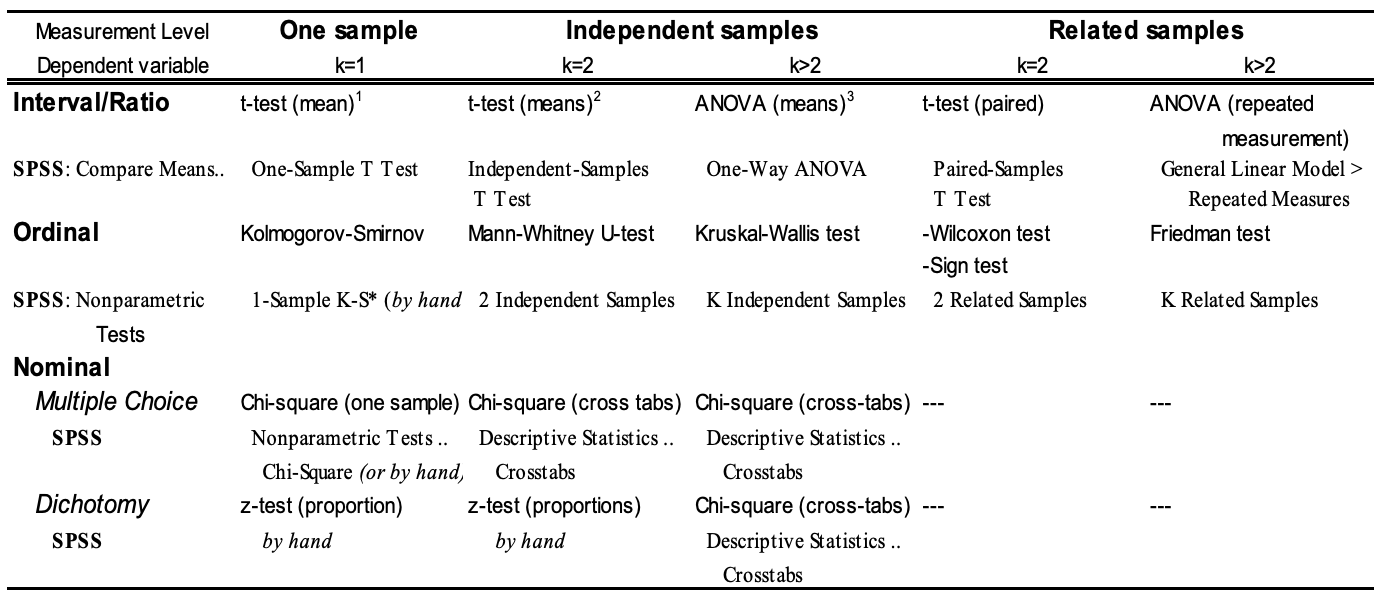
\includegraphics{../assets/test-by-variable-type.png}

    \subsection{Z-Test}

    \paragraph{Procedure} Calculate the z-value and the p-value(two-sided and one-sided). Compare computed z-statistic to critical value of z:
    2-sided test (testing equality): 1.96 for sign. level 0.05, 1.65 for sign. level 0.1;
    1-sided test (greater or smaller than): 1.65 for sign level 0.05, 1.29 for sign. level 0.1
    If absolute value of z-statistic > critical value of z $\rightarrow$ H_0 (equality) is rejected at given sign level

    \paragraph{\textit{Example}} \textit{
    Comparing the proportion of a dichotomous variable (yes/no) to a
    specific value in one sample (e.g., is the choice of the brand in the
    sample equal to 50\%?). Given is $p=0.63$, $n=141$ $\rightarrow$ \textbf{Nominal Measurement of one-sample}

    $\pi=0.5$; $p=0.603$; $n=141$ $\rightarrow$ $z=2.45$

    Abs. value of z-test > critical value of 1.96 (so p < .05) $\rightarrow$ H0 is rejected, proportion of men in the sample is different from 50\%
    }

    \subsection{T-Test}

    \paragraph{\textit{Example}} \textit{
    According to official statistics, the average household size in the population in the Netherlands is 2.28.
    Given that $T=5.99$, $n=140$, $\sigma = 0$
    The mean in the sample is 2.92. Is the sample representative of the population?

    $\rightarrow$ \textbf{Interval Measurement of one-sample}
    
    $H_0$: mean in the population where the sample came from = 2.28.
    
    $\sigma < 0.05 \rightarrow H_0$ is rejected $\rightarrow$ mean household size in the sample is significantly different from 2.28
    }

    \subsection{Kolmogorov Smrnoc}

    \paragraph{\textit{Example}} \textit{
    Household size = 1: 34.4\%, Household size = 2: 32.7\%, Household size = 3: 12.8\%, Household size = 4: 13.7\%, Household size > 5: 6.4\%
    Is the sample representative of the population?

    $\rightarrow$ \textbf{Ordinal Measurement of one-sample}
    
    $H_0$: are the proportions of respondents in the population where the sample came from equal to the ones provided in the statistics report?

    Compare observed distribution with distribution total population. Test statistic = largest absolute difference in cummultative percentages $K = 0.23$
    Critical Value at 5\% = $\frac{P(0.23 | H_0 true)}{\sqrt{n}} = \frac{1.36}{\sqrt{141}} = 0.11$
    $P(0.23 | H_0 true) > CV(0.11) \rightarrow H_0$ is rejected $\rightarrow$ the sample proportions are different from given population proportions, the sample is not representative.
    }

    \subsection{ANOVA}
    
    \paragraph{\textit{Example}} \textit{
    Do women like branded beers as much as men? Assuming equal variances. 

    $\rightarrow$ \textbf{Interval Measurement of two-sample (k>2)}

    $H_0$: for each branded beer, women's mean liking = men's mean liking

    $t_1 = -0.482$, $\sigma_1 = 0.631$, $t_2 = 0.57$, $\sigma_2 = 0.57$
    $p > 0.1 \rightarrow H_0$ is not rejected $\rightarrow$ women's liking of branded beers is not different from men's.
    }
    
    \paragraph{\textit{Example}} \textit{
    Do consumers in different regions (big cities, south, west, and east) like each beer equally?

    $\rightarrow$ \textbf{ liking of each beer is equal across regions}

    $H_0$:  liking of each beer is equal across regions

    For evaluations of brand B, p < .05 - Liking of brand B differ across regions. 
    Post-Hoc: Which region differs the most in liking of brand B?

    $t_1 = -0.482$, $\sigma_1 = 0.631$, $t_2 = 0.57$, $\sigma_2 = 0.57$
    $p > 0.1 \rightarrow H_0$ is not rejected $\rightarrow$ women's liking of branded beers is not different from men's.
    }
    
%    Todo: make this section better
    

\end{section}
